% *********************************************************************
% © 2010–2023 Jeremy Sylvestre
%
% Permission is granted to copy, distribute and/or modify this document
% under the terms of the GNU Free Documentation License, Version 1.3 or
% any later version published by the Free Software Foundation; with no
% Invariant Sections, no Front-Cover Texts, and no Back-Cover Texts. A
% copy of the license is included in the appendix entitled “GNU Free
% Documentation License” that appears in the output document of this
% PreTeXt source code. All trademarks™ are the registered® marks of
% their respective owners.
%
% *********************************************************************

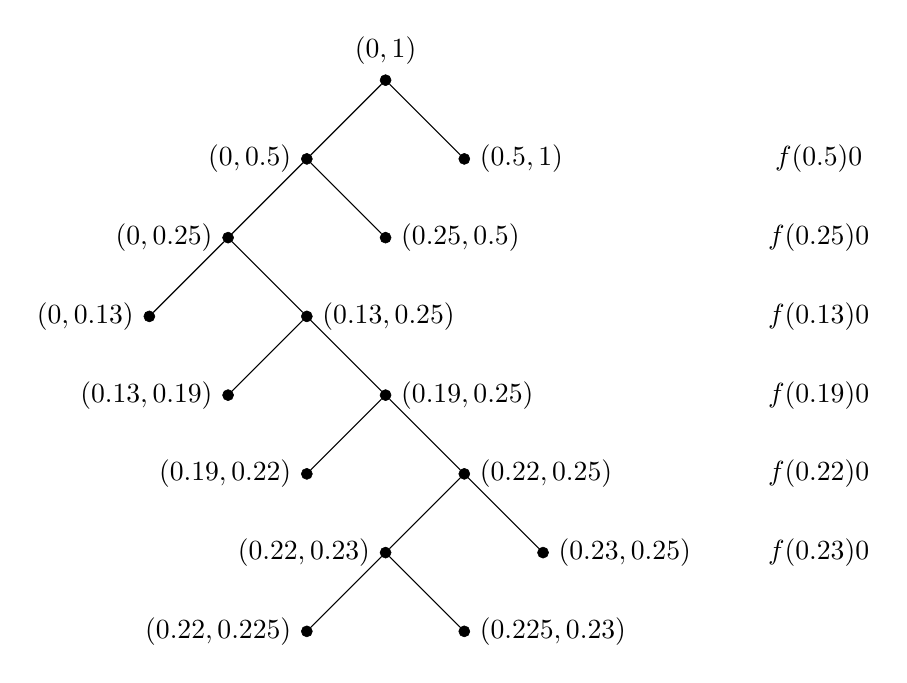
\begin{tikzpicture}[
	vertex/.style={ circle, draw, very thin, fill, inner sep=0pt, minimum size=4pt },
	vertexg/.style={ black!40!white, circle, draw, very thin, fill, inner sep=0pt, minimum size=4pt },
	vertexo/.style={ circle, draw, very thin, inner sep=0pt, minimum size=4pt }
]

\node at (0,0) (start) [vertex,label=above:{$(0,1)$}] {};

\node at (-1,-1) (c1v1) [vertex,label=left:{$(0,0.5)$}] {};
\node at (1,-1) (c1v2) [vertex,label=right:{$(0.5,1)$}] {};
\foreach \p in {c1v1,c1v2} \draw (start) to (\p);

\node at (5.5,-1) {$f(0.5) \gt 0$};

\node at (-2,-2) (c2v1) [vertex,label=left:{$(0,0.25)$}] {};
\node at (0,-2) (c2v2) [vertex,label=right:{$(0.25,0.5)$}] {};
\foreach \p in {c2v1,c2v2} \draw (c1v1) to (\p);

\node at (5.5,-2) {$f(0.25) \gt 0$};

\node at (-3,-3) (c3v1) [vertex,label=left:{$(0,0.13)$}] {};
\node at (-1,-3) (c3v2) [vertex,label=right:{$(0.13,0.25)$}] {};
\foreach \p in {c3v1,c3v2} \draw (c2v1) to (\p);

\node at (5.5,-3) {$f(0.13) \lt 0$};

\node at (-2,-4) (c4v1) [vertex,label=left:{$(0.13,0.19)$}] {};
\node at (0,-4) (c4v2) [vertex,label=right:{$(0.19,0.25)$}] {};
\foreach \p in {c4v1,c4v2} \draw (c3v2) to (\p);

\node at (5.5,-4) {$f(0.19) \lt 0$};

\node at (-1,-5) (c5v1) [vertex,label=left:{$(0.19,0.22)$}] {};
\node at (1,-5) (c5v2) [vertex,label=right:{$(0.22,0.25)$}] {};
\foreach \p in {c5v1,c5v2} \draw (c4v2) to (\p);

\node at (5.5,-5) {$f(0.22) \lt 0$};

\node at (0,-6) (c6v1) [vertex,label=left:{$(0.22,0.23)$}] {};
\node at (2,-6) (c6v2) [vertex,label=right:{$(0.23,0.25)$}] {};
\foreach \p in {c6v1,c6v2} \draw (c5v2) to (\p);

\node at (5.5,-6) {$f(0.23) \gt 0$};

\node at (-1,-7) (c7v1) [vertex,label=left:{$(0.22,0.225)$}] {};
\node at (1,-7) (c7v2) [vertex,label=right:{$(0.225,0.23)$}] {};
\foreach \p in {c7v1,c7v2} \draw (c6v1) to (\p);

\end{tikzpicture}
